%!TEX program = xelatex

\documentclass[a4paper, openany, oneside]{memoir}
\usepackage[no-math]{fontspec}
\usepackage{pgfplots}
\usepackage{float}
\pgfplotsset{compat=newest}
\usepackage{commath}
\usepackage{mathtools}
\usepackage{amssymb}
\usepackage{amsthm}
\usepackage{booktabs}
\usepackage{todonotes}
\usepackage{mathtools}
\usepackage{xcolor}
\usepackage[separate-uncertainty=true, per-mode=symbol]{siunitx}
\usepackage{listings}
\usepackage[american inductor, european resistor]{circuitikz}
\usepackage{amsmath}
\usepackage{amsfonts}
\usepackage{ifxetex}
\usepackage[dutch,english]{babel}
\usepackage[backend=bibtexu,texencoding=utf8,bibencoding=utf8,style=ieee,sortlocale=en_GB,language=auto]{biblatex}
\usepackage[strict,autostyle]{csquotes}
\usepackage{import}
\usepackage{standalone}
\usepackage{bookmark,hyperref}
\usepackage{xcolor,mdframed}
\usepackage{tikz}
\usepackage{framed}
\usepackage{float}
\usepackage{tabularx}
\usepackage{graphicx,adjustbox}
\usepackage{rotating}
\usepackage{pdfpages}
\usepackage{enumitem}
\usepackage{calc}
\usepackage{pgfplots}
\usepackage{filecontents}
\usepackage{caption}
\usepackage{subcaption}
\usepackage{lettrine}

\newcolumntype{Y}{>{\raggedright\arraybackslash}X} % Left-justified text in tabularx environment

\ifxetex{} % Fonts laden in het geval dat je met Xetex compiled
    \usepackage{fontspec}
    \defaultfontfeatures{Scale=MatchLowercase, Ligatures=TeX} % To support LaTeX quoting style
    %\setromanfont{Palatino Linotype} % Tover ergens in Font mapje in root.
    \setsansfont{Avenir Next LT Pro}
    \setromanfont{Adobe Caslon Pro} % Tover ergens in Font mapje in root.
    \setmonofont{Source Code Pro}
\else % Terug val in standaard pdflatex tool chain. Geen ondersteuning voor OTT fonts
    \usepackage[T1]{fontenc}
    \usepackage[utf8]{inputenc}
\fi
\usepackage[noabbrev, capitalize]{cleveref}
\usepackage{ifthen}
\usepackage{titlesec}
\usepackage{titlecaps}

\newcommand{\references}[1]{\begin{flushright}{#1}\end{flushright}}
\renewcommand{\vec}[1]{\boldsymbol{\mathbf{#1}}}
\newcommand{\uvec}[1]{\boldsymbol{\hat{\vec{#1}}}}
\newcommand{\mat}[1]{\boldsymbol{\mathbf{#1}}}
\newcommand{\fasor}[1]{\boldsymbol{\tilde{\vec{#1}}}}
\newcommand{\cmplx}[0]{\mathrm{j}}
\renewcommand{\Re}[0]{\operatorname{Re}}
\newcommand{\Cov}{\operatorname{Cov}}
\newcommand{\Var}{\operatorname{Var}}
\newcommand{\proj}{\operatorname{proj}}
\newcommand{\Perp}{\operatorname{perp}}
\newcommand{\col}{\operatorname{col}}
\newcommand{\rect}{\operatorname{rect}}
\newcommand{\sinc}{\operatorname{sinc}}
\newcommand{\lcm}{\operatorname{lcm}}
%\newcommand{\gcd}{\operatorname{gcd}}
\newcommand{\F}{\mathcal{F}}
\newcommand{\DTFT}{\mathcal{F}_*}
\newcommand{\conj}[1]{#1^*}
\renewcommand{\mod}{\operatorname{mod}}
\newcommand{\rot}{\operatorname{rot}}
\newcommand{\vecsc}[1]{\vec{\textsc{\textbf{#1}}}}
\renewcommand{\ss}[1]{_{#1}}

% Label without linebreak breaker
\newcommand{\lab}[1]{\label{#1}\nolinebreak}

\newtheorem{definition}{Definition}
\newtheorem{theorem}{Theorem}


\DeclareSIUnit{\voltampere}{VA} %apparent power
\DeclareSIUnit{\pii}{\ensuremath{\pi}}

\hypersetup{%setup hyperlinks
    colorlinks,
    citecolor=black,
    filecolor=black,
    linkcolor=black,
    urlcolor=black
}

% Example boxes
\usepackage{fancybox}
\usepackage{framed}
\usepackage{adjustbox}
\newenvironment{simpages}%
{\AtBeginEnvironment{itemize}{\parskip=0pt\parsep=0pt\partopsep=0pt}
\def\FrameCommand{\fboxsep=.5\FrameSep\shadowbox}\MakeFramed{\FrameRestore}}%
{\endMakeFramed}

% Impulse train
\DeclareFontFamily{U}{wncy}{}
\DeclareFontShape{U}{wncy}{m}{n}{<->wncyr10}{}
\DeclareSymbolFont{mcy}{U}{wncy}{m}{n}
\DeclareMathSymbol{\Sha}{\mathord}{mcy}{"58}

\setlength{\parindent}{0pt}
\nonzeroparskip

% Block environment configuration
\newcommand{\BlockLeftMargin}{20pt}
\newcommand{\BlockLeftMarginText}{25pt}
\newcommand{\BlockLeftMarginTextSpacing}{10pt}

% Own colours
\definecolor{gray75}{gray}{0.75}

% Block environment
\newenvironment{block}[3]{%
\makebox{\hspace{-\spinemargin}%
\begin{tikzpicture}[overlay]
    \draw [thick,color=gray75] (\BlockLeftMargin, 0) -- (\paperwidth - \spinemargin, 0);
    \node at (\BlockLeftMarginText, -0.9) [align=left, text width=\spinemargin - \BlockLeftMarginText - \BlockLeftMarginTextSpacing, anchor=west, text depth=1cm] {\textbf{\textsc{#1}}\newline\textit{#3}};
\end{tikzpicture}}%
\nopagebreak\\[0.25em]\ifthenelse{\equal{#2}{}}{}{(\textit{#2}.) }\nopagebreak\nolinebreak}
{\nopagebreak\\[-0.25em]%
\makebox{\hspace{-\spinemargin}%
\begin{tikzpicture}[overlay, remember picture]
    \draw [thick,color=gray75] (\spinemargin,0) -- (\paperwidth - \spinemargin,0);
\end{tikzpicture}} \vspace{0.5em}}

% Theorem
\newcounter{blockTheoremCounter}
\crefname{blockTheoremCounter}{Theorem}{Theorems}
\Crefname{blockTheoremCounter}{Theorem}{Theorems}

\newenvironment{blockTheorem}[1][]{%
\refstepcounter{blockTheoremCounter}%
\begin{block}{theorem \theblockTheoremCounter}{#1}{}}
{\end{block}}

% Definition
\newcounter{blockDefinitionCounter}
\crefname{blockDefinitionCounter}{Definition}{Definitions}
\Crefname{blockDefinitionCounter}{Definition}{Definitions}

\newenvironment{blockDefinition}[1][]{%
\refstepcounter{blockDefinitionCounter}%
\begin{block}{definition \theblockDefinitionCounter}{#1}{}}
{\end{block}}

% Proof
\newcounter{blockProofTheoremCounter}
\crefname{blockProofTheoremCounter}{Proof}{Proofs}
\Crefname{blockProofTheoremCounter}{Proof}{Proofs}

\newenvironment{blockProofTheorem}[1]{%
\refstepcounter{blockProofTheoremCounter}%
\begin{block}{proof of \\ theorem #1}{}{}}
{\qed\end{block}}

% Detail
\newcounter{blockDetailCounter}
\crefname{blockDetailCounter}{Detail}{Details}
\Crefname{blockDetailCounter}{Detail}{Details}

\newenvironment{blockDetail}[1][]{%
\refstepcounter{blockDetailCounter}%
\begin{block}{detail \theblockDetailCounter}{#1}{}}
{\end{block}}

% Redesign chapter headings
\newcommand{\chapternumber}{\thechapter}
\newcommand{\hsp}{\hspace{20pt}}
\titleformat{\chapter}[hang]{\Huge\bfseries}{\chapternumber\hsp\textcolor{gray75}{|}\hsp}{0pt}{\Huge\bfseries}

% Remove headers
% \addtopsmarks{headings}{}{
%   \createmark{chapter}{left}{nonumber}{}{}
% }
% \pagestyle{headings} % Activate changes

% Capitalise headers in a regular way
\renewcommand*{\memUChead}[1]{\titlecap{#1}}

% \hfill for math mode
\newcommand{\pushright}[1]{\intertext{\hfill$\displaystyle #1$}}
\newcommand{\pushline}{\hskip \textwidth minus \textwidth}
\newcommand{\matlab}{\textsc{Matlab}}

\definecolor{code-grey}{HTML}{DDDDDD}
\newcommand{\lib}[1]{\textsf{#1}}
\newcommand{\file}[1]{\textsf{#1}}
\newcommand{\func}[1]{\colorbox{code-grey}{\texttt{#1}}}
\newcommand{\class}[1]{\colorbox{code-grey}{\texttt{#1}}}

% Setup actiepunten
\newenvironment{important}[1][]{%
   \begin{mdframed}[%
      backgroundcolor={red!15}, hidealllines=true,
      skipabove=0.7\baselineskip, skipbelow=0.7\baselineskip,
      splitbottomskip=2pt, splittopskip=4pt, #1]%
   \makebox[0pt]{% ignore the withd of !
      \smash{% ignor the height of !
         \fontsize{32pt}{32pt}\selectfont% make the ! bigger
         \hspace*{-19pt}% move ! to the left
         \raisebox{-2pt}{% move ! up a little
            {\color{red!70!black}\sffamily\bfseries !}% type the bold red !
         }%
      }%
   }%
}{\end{mdframed}}
\newcommand{\excl}[1]{
\begin{important}
  \textbf{#1}
\end{important}
}

\makeatletter
\newcommand\footnoteref[1]{\protected@xdef\@thefnmark{\ref{#1}}\@footnotemark}
\makeatother

% Allow page breaks in display environments
%\allowdisplaybreaks
% S unit for use in Mega Samples per second
\DeclareSIUnit\sample{S}

\newcommand{\CC}{C\nolinebreak\hspace{-.05em}\raisebox{.3ex}{ \textbf{+}}\nolinebreak\hspace{-.10em}\raisebox{.3ex}{\textbf{+}}}
\def\CC{{C\nolinebreak[4]\hspace{-.05em}\raisebox{.3ex}{\textbf{++}}}}


\newcommand{\partauthor}[1]{\gdef\@partauthor{#1}}
\renewcommand{\printparttitle}[1]{
  \parttitlefont #1\\
  \vspace{1.5cm}
  \textnormal{\Large \@partauthor}
}
\addbibresource{../../../../includes/bibliography.bib}

\begin{document}

% \section{Concept}
The first step of spectrum sensing is sampling the signal. Conventional methods sample at a uniform sample rate to ensure complete reconstruction of the signal. With uniform sampling, every subsequent sample has an equal delay in time. This is illustrated by \cref{tkz:uniform}.

\begin{figure}[H]
\centering
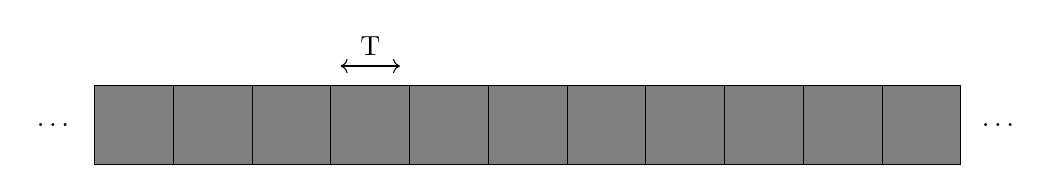
\begin{tikzpicture}

\draw [fill=gray]  (-2,0) rectangle (-1,-1);
\draw [fill=gray]  (-1,0) rectangle (0,-1);
\draw [fill=gray]  (0,0) rectangle (1,-1);
\draw [fill=gray]  (1,0) rectangle (2,-1);
\draw [fill=gray]  (2,0) rectangle (3,-1);
\draw [fill=gray]  (3,0) rectangle (4,-1);
\draw [fill=gray]  (4,0) rectangle (5,-1);
\draw [fill=gray]  (5,0) rectangle (6,-1);
\draw [fill=gray]  (6,0) rectangle (7,-1);
\draw [fill=gray]  (7,0) rectangle (8,-1);
\draw [fill=gray]  (8,0) rectangle (9,-1);

\node (v1) at (-2.5,-.5) {};
\node (v2) at (9.5,-.5) {};
\draw  (v1) node {\dots} ;
\draw  (v2) node {\dots} ;

\node (v3) at (1,.25) {};
\node (v4) at (2,.25) {};
\draw  [<->] (v3) edge (v4);

\node (v5) at (1.5,.5) {};
\draw  (v5) node {T} ;
\end{tikzpicture}
\caption{Uniform sampling with sample period T. Gray blocks are sampled}\label{tkz:uniform}
\end{figure}

When one desires to ensure full reconstruction of the signal with uniform sampling one needs to sample at the Nyquist rate \todo{ref}. However, we don't need a full recovery of the signal, but are only interested in certain properties of the signal. To improve our sampling methods we remove the restriction of uniform sampling to look for more efficient ways to sample the spectrum, and efficiently recover the information we are looking for. Non uniform sampling has no restriction on delays of subsequent samples as is illustrated in \cref{tkz:nonuniform}.

\begin{figure}[H]
\centering
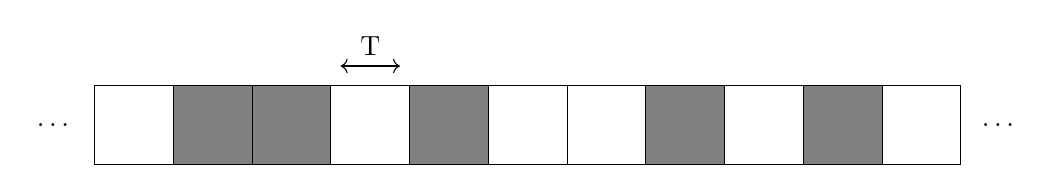
\begin{tikzpicture}

\draw  (-2,0) rectangle (-1,-1);
\draw [fill=gray]  (-1,0) rectangle (0,-1);
\draw [fill=gray]  (0,0) rectangle (1,-1);
\draw  (1,0) rectangle (2,-1);
\draw [fill=gray] (2,0) rectangle (3,-1);
\draw  (3,0) rectangle (4,-1);
\draw  (4,0) rectangle (5,-1);
\draw [fill=gray]  (5,0) rectangle (6,-1);
\draw  (6,0) rectangle (7,-1);
\draw  [fill=gray] (7,0) rectangle (8,-1);
\draw  (8,0) rectangle (9,-1);

\node (v1) at (-2.5,-.5) {};
\node (v2) at (9.5,-.5) {};
\draw  (v1) node {\dots} ;
\draw  (v2) node {\dots} ;

\node (v3) at (1,.25) {};
\node (v4) at (2,.25) {};
\draw  [<->] (v3) edge (v4);

\node (v5) at (1.5,.5) {};
\draw  (v5) node {T} ;
\end{tikzpicture}
\caption{Non-uniform sampling with sample period T. Gray blocks are sampled}\label{tkz:nonuniform}
\end{figure} 

This is however not trivial to implement on a device. To perform non-uniform sampling we introduce multi-coset sampling. Multi-coset sampling is a set of sampling methods that use multiple samplers, or cosets, to sample the spectrum. This is illustrated in \cref{tkz:multicoset}

\begin{figure}[H]
\centering
\begin{tikzpicture}
\draw  (-2.5,2) rectangle (-1.5,1) node[pos=.5]{$x$};
\draw  (-1.5,1.5) -- (0.5,1.5);
\draw  (-0.5,3) -- (0.5,3);
\draw (-0.5,3) -- (-0.5,-0.5);

\node at (2.5,-.91) {\vdots};
\node at (0.75,-.91) {\vdots};
\node at (-0.5,-.91) {\vdots};

\draw (-0.5,-1.5) -- (-0.5,-2);
\draw  (1,3) -- (2,3);
\draw  (1,1.5) -- (2,1.5);
\draw  (1,0) -- (2,0);
\draw  (1,-2) -- (2,-2);
\draw (-0.5,0) -- (0.5,0);
\draw (-0.5,-2) -- (0.5,-2);
\draw[ very thick](0.5,3)-- +(30:0.46);
\draw[ very thick](0.5,1.5)-- +(30:0.46);
\draw[ very thick](0.5,0)-- +(30:0.46);
\draw[ very thick](0.5,-2)-- +(30:0.46);
\draw  (3,2) rectangle (2,1) node[pos=.5]{$y_1$};
\draw  (3,0.5) rectangle (2,-0.5) node[pos=.5]{$y_2$};
\draw  (3,-1.5) rectangle (2,-2.5) node[pos=.5]{$y_m$};
\draw  (3,3.5) rectangle (2,2.5) node[pos=.5]{$y_0$};
\end{tikzpicture}
\caption{schematic multi-coset sampling with $m$ cosets}\label{tkz:multicoset}
\end{figure}

In the reconstruction section we will deduce criteria on the sampling that will further specify the samplers. In the sampling section methods we will then get back to multi-coset sampling to link it to the reconstruction and optimize performance.

\end{document}

